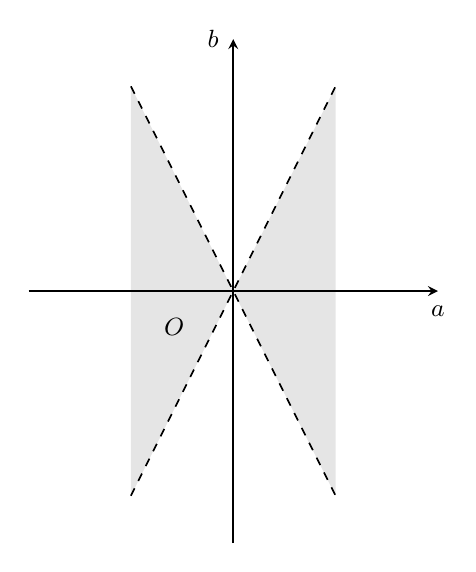
\begin{tikzpicture}[scale=1,line width=.6pt]
\tikzset{lbl/.style={font=\small,inner sep=1pt}}
% Side regions bounded by the two dashed lines.
\fill[gray!20] (-1.3,-2.6)--(-1.3,2.6)--(0,0)--cycle;
\fill[gray!20] (1.3,-2.6)--(1.3,2.6)--(0,0)--cycle;
% axes
\draw[->,>=stealth] (-2.6,0)--(2.6,0) node[lbl,below=4pt] at (2.6,0) {$a$};
\draw[->,>=stealth] (0,-3.2)--(0,3.2) node[lbl,left=4pt] at (0,3.2) {$b$};
% dashed boundary b=+-2a
\draw[dashed] (-1.3,-2.6)--(1.3,2.6);
\draw[dashed] (-1.3,2.6)--(1.3,-2.6);
\node[lbl] at (-0.75,-0.45) {$O$};
\end{tikzpicture}